\documentclass[tikz]{standalone}
\usepackage{amsmath}
\usepackage{xcolor}
\usetikzlibrary{calc}
\definecolor{bg}{HTML}{171D2B}
\definecolor{aksen}{HTML}{F7B538}
\definecolor{teks}{HTML}{FFFFFF}
\begin{document}
\pagecolor{bg}
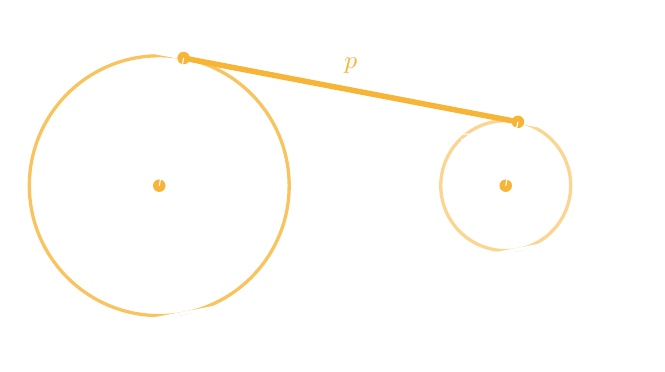
\begin{tikzpicture}[
  scale=0.55,
  every node/.style={text=teks, font=\small},
  dot/.style={circle, fill=aksen, inner sep=1.6pt}
]
  % Lingkaran 1: pusat A, jari-jari 3
  \coordinate (A) at (0,0);
  % Lingkaran 2: pusat B, jari-jari 1.5, jarak AB = 8
  \coordinate (B) at (8,0);
  \draw[very thick, aksen!80] (A) circle (3);
  \draw[very thick, aksen!55] (B) circle (1.5);
  % Titik singgung (normal n = (0.1875, 0.98231))
  \coordinate (P1) at (0.5625, 2.9469);   % di lingkaran besar, atas
  \coordinate (P2) at (8.28125, 1.4735);  % di lingkaran kecil, atas
  \coordinate (Q1) at (0.5625, -2.9469);  % bawah
  \coordinate (Q2) at (8.28125, -1.4735);
  % Garis singgung persekutuan luar
  \draw[white, very thick] ($(P1)!-0.45!(P2)$) -- ($(P2)!-0.35!(P1)$);
  \draw[white, very thick] ($(Q1)!-0.45!(Q2)$) -- ($(Q2)!-0.35!(Q1)$);
  % Segmen singgung P1P2 di-highlight
  \draw[aksen, line width=2pt] (P1) -- (P2);
  % Pusat dan segmen penghubung
  \draw[dashed, teks!60] (A) -- (B);
  \node[dot, label={below left:$A$}] at (A) {};
  \node[dot, label={below right:$B$}] at (B) {};
  \node[dot] at (P1) {}; \node[dot] at (P2) {};
  \node[text=aksen, above] at ($(P1)!0.5!(P2)+(0,0.15)$) {$p$};
  % Label jari-jari
  \draw[teks!70] (A) -- (0.5625,2.9469);
  \node[teks!80] at (0.2,1.9) {$R=3$};
  \draw[teks!70] (B) -- (8.28125,1.4735);
  \node[teks!80] at (7.4,1.1) {$r=1{,}5$};
  % Label jarak pusat
  \node[below, teks!80] at (4,-0.15) {$d=8$};
\end{tikzpicture}
\end{document}
